\documentclass[dvipsnames, tikz]{standalone}
\usepackage{tikz}
\usetikzlibrary{positioning}

\begin{document}

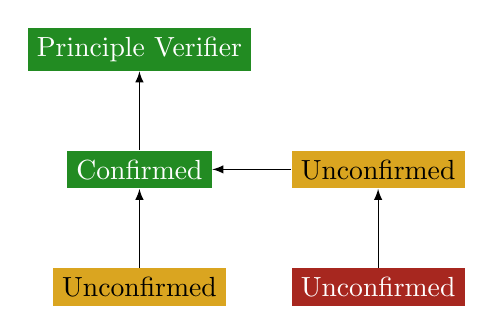
\begin{tikzpicture}
  [
    -latex,
    confirmed/.style={text=white, fill=ForestGreen},
    unconfirmed/.style={fill=Goldenrod},
    illegal/.style={text=white, fill=Mahogany}
  ]

  \node[confirmed] (pv) {Principle Verifier};
  \node[confirmed] (c) [below=of pv] {Confirmed};
  \node[unconfirmed] (uc1) [below=of c] {Unconfirmed};
  \node[unconfirmed] (uc2) [right=of c] {Unconfirmed};
  \node[illegal] (i) [below=of uc2] {Unconfirmed};

  \draw (c) -- (pv);
  \draw (uc1) -- (c);
  \draw (uc2) -- (c);
  \draw (i) -- (uc2);

\end{tikzpicture}

\end{document}
